\chapter{Design}\label{design}

%------------------------------------------------------
\section{Architecture}

The project is divided into the \texttt{import} phase where
the ETL process  happens and an \texttt{export} phase where the PostGIS data
is transformed into vector tiles using the \texttt{open-streets} data style.
The data style depends on the database schema defined by the \texttt{import}.
\\\\
Along the way many additional development \texttt{tooling} was needed for the reverse engineering process and for improving developer productivity. Everything that is not needed during
the workflow but only for development or verification is in this package.
\\\\
The infrastructure package contains specially configured programs as Docker images.
It contains a PostGIS database, a connection pooler (pgbouncer) and a tessera based raster tile server.

\begin{figure}[h]
  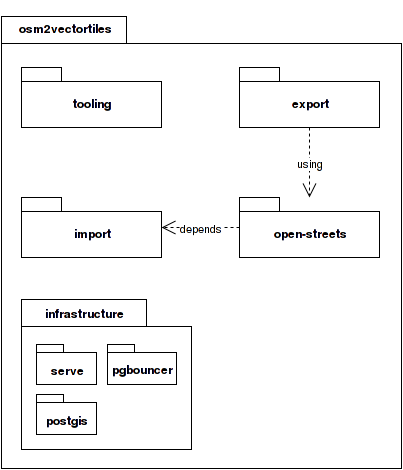
\includegraphics[scale=0.6]{images/high_level_packages.png}
  \caption{High level package diagram}
\end{figure}

%------------------------------------------------------
\newpage
\subsection{Import}

The import consists of several imports of different data sources.

\paragraph{import-osm-data}
Import of the OSM planet file with a custom mapping configuration.

\paragraph{import-sql}
Custom SQL functions to keep SQL queries in the \texttt{open-streets} data style DRY and generated SQL code for classifications. 

\paragraph{update-scaleranks}
Custom scalerank updates from Natural Earth data for better scaleranks in places.

\paragraph{import-natural-earth}
Import of Natural Earth data.

\paragraph{import-water}
Water polygons from OpenStreetMapData.

\paragraph{import-labels}
Custom curated labels for marine, countries and states.

\begin{figure}[h]
  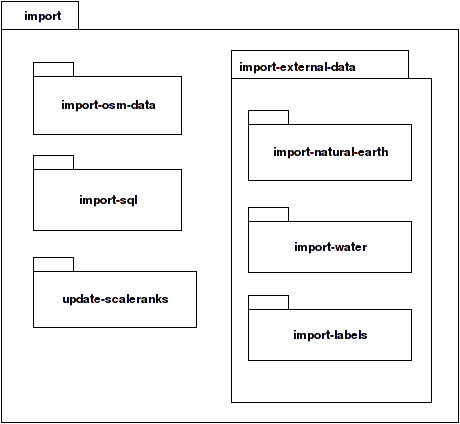
\includegraphics[scale=0.6]{images/import_all_package_diagram.png}
  \caption{Import package}
\end{figure}


%------------------------------------------------------
\newpage
\subsection{Export}
Export can either be done locally which will process one bounding box or in parallel on several
remote machines. In this thesis we will only focus on local export.


\paragraph{open-streets}
The data style project is the most essential component which pulls together all the
data of different datasources to create vector tiles. 

\paragraph{export-local}
A process which is using the open-streets.tm2source project to create vector tiles for a
given bounding box.

\paragraph{export-remote}
A worker implementation which uses a queue to read jobs and work through jobs with
\texttt{export-local}.

\begin{figure}[h]
  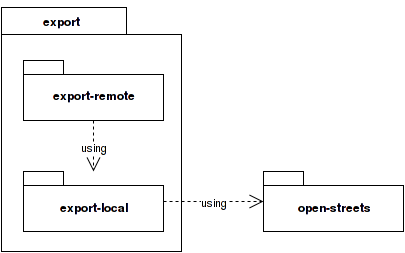
\includegraphics[scale=0.6]{images/export_package.png}
  \caption{Export package}
\end{figure}
\newpage

%------------------------------------------------------
\newpage
\subsection{Tooling}

This chapter describes the various tools we created to support the development process.

\paragraph{enqueue-jobs}
Create jobs for certain areas automatically.

\paragraph{merge}
Merge results of jobs together into a final big file.

\paragraph{verify}
Verify size and correctness of MBTiles files.

\paragraph{compare}
Compare different vector tiles for their differences.

\paragraph{visual-compare}
Compare different raster tiles in an interactive map.

\paragraph{generate-diagrams}
Generate mapping and layer diagrams from source code.

\paragraph{test-performance}
Load testing with Gatling for tileserver implementation.

\paragraph{mapbox-studio}
Mapbox studio in a Docker container for working on a server.

\paragraph{optimize-mbtiles}
Remove redundant subpyramids of MBTiles to save disk space.

\begin{figure}[h]
  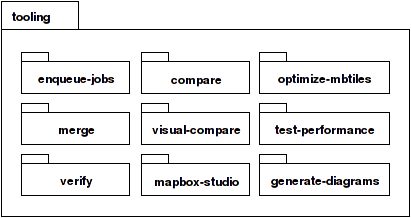
\includegraphics[scale=0.6]{images/tooling_package_diagram.png}
  \caption{Tooling package}
\end{figure}

%------------------------------------------------------
\newpage
\section{Deployment}\label{deployment}

All workflow processes are deployed as Docker containers. The software package
is usually one single process.

\subsection{Import}

The data container pattern\footnote{\url{http://container42.com/2013/12/16/persistent-volumes-with-docker-container-as-volume-pattern/}} is used in \texttt{cache} and \texttt{pgdata}. Those
data only containers are mounted from \texttt{import-osm-data} for storing cache data while importing and in the \texttt{postgis} for storing the database files.
For convenience the \texttt{import-external-data} imports several data sources at once.

\begin{figure}[h]
  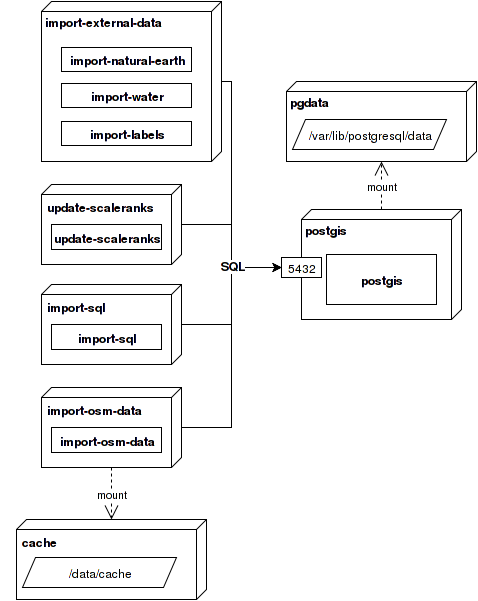
\includegraphics[scale=0.6]{images/deployment_import.png}
  \caption{Import deployment diagram}
\end{figure}

%------------------------------------------------------
\newpage
\subsection{Export and Development Tools}

For performance reason a connection pooler is in front of the actual \texttt{postgis} container.
\\
The raster tile server can serve directly from the export directory where the generated MBTiles
are put. The \texttt{mapbox-studio} container allows editing the \texttt{open-streets} project and connects directly to the \texttt{postgis} container.

\begin{figure}[h]
  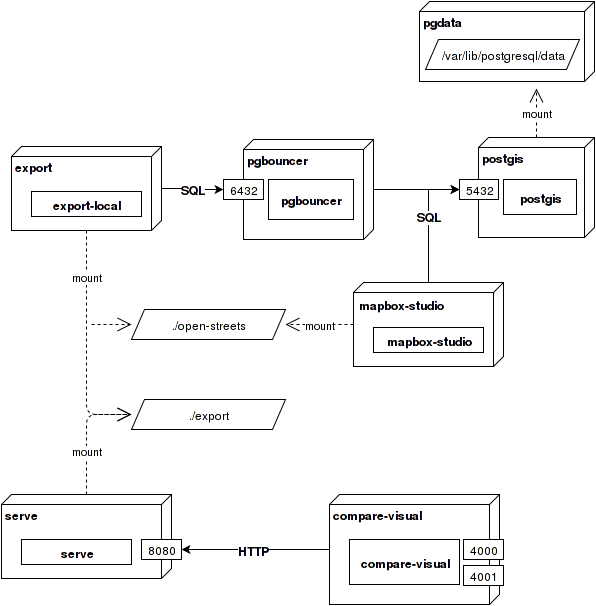
\includegraphics[scale=0.6]{images/deployment_dev_export.png}
  \caption{Export and development tools deployment diagram}
\end{figure}

%------------------------------------------------------
\newpage
\section{Workflow}\label{workflow}

\subsection{Import}\label{workflow-import}

\begin{figure}[h]
  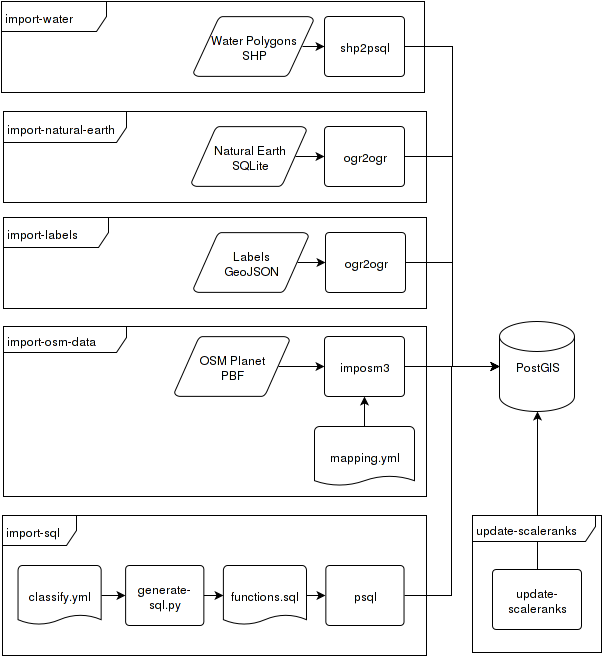
\includegraphics[scale=0.6]{images/import_package_flow.png}
  \caption{Import workflow from various data sources into PostGIS}
\end{figure}

\newpage
\subsection{Export}\label{workflow-export}

For generating the vector tiles the tilelive tool \texttt{tl} \footnote{\url{https://github.com/mojodna/tl}} is used which wraps
around Mapnik. 
\marginpar{\nameref{data_style} is a Mapbox Studio source project.}
The data style defines all feature sets (layers) and is transformed into a Mapnik
XML stylesheet.

The \texttt{tl} utility stores the generated vector tiles in a MBTiles container.

\begin{figure}[h]
  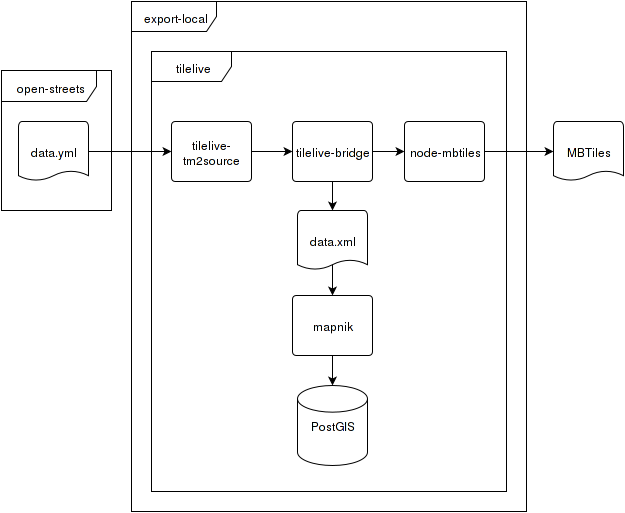
\includegraphics[scale=0.6]{images/export_package_flow.png}
  \caption{Export data from PostGIS to MBTiles}
\end{figure}

%------------------------------------------------------
\newpage
\section{Database Schema}\label{database-schema}
The schema is flat and has no relations. Each table contains information about its entity and geometry. 

\subsection{OpenStreetMap Planet}

The cornerstone of the entire map is \osm{} data from published snapshots from OSM Planet\footnote{\url{http://planet.osm.org/}}.
\marginpar{The OSM data is perfect for high zoom levels where detailed coverage of local areas is important.}
Smaller extracts for single countries and continents are available from Geofabrik\footnote{\url{http://download.geofabrik.de/}}.
For  single cities or regions the Metro extracts from Mapzen\footnote{\url{https://mapzen.com/data/metro-extracts/}} can be used.
\\
The data is available in the PBF\footnote{\url{http://wiki.openstreetmap.org/wiki/PBF_Format}} and OSM XML format \footnote{\url{https://wiki.openstreetmap.org/wiki/OSM_XML}}. 
Data in PBF format is 30\% smaller and 5-6 times faster to read and write than the bzipped OSM XML version.
\\
We use imposm3 to import the OSM data into our PostGIS database.
Selected tags \footnote{\url{http://wiki.openstreetmap.org/wiki/Tags}} and their geometries are defined in an import mapping explicitly.
Because imposm3 cannot match two types of polygons (e.g. polygon and point) we need
to create a table for each geometry type.

\begin{flushleft}
    \begin{tabular}{lll}
    \hline
    Table Name            & Geometry Type & Description \\
    \hline                                          
    admin                  & linestring    & Administrative boundaries \\
    buildings              & polygon       & Building shapes                            \\
    landusages             & polygon       & Human use of land \\
    places                 & point         & Populated settlements                      \\
    roads                  & linestring    & Roads, tracks and paths          \\
    aero\_lines            & linestring    & Airports and aviation-related items        \\
    aero\_polygons         & polygon       & see aero\_lines                            \\
    barrier\_lines         & linestring    & Movement blocking structures   \\
    barrier\_polygons      & polygon       & see barrier\_lines                         \\
    housenumbers\_points   & point         & Address information about houses \\
    housenumbers\_polygons & polygon       & see housenumbers\_points                   \\
    poi\_points            & point         & Point of interest                          \\
    poi\_polygons          & polygon       & see poi\_points                            \\
    water\_lines           & linestring    & Lakes and rivers                           \\
    water\_polygons        & polygon       & see water\_lines                           \\
    \end{tabular}
\end{flushleft}

\subsection{Custom Curated Labels}

The placement and importance of labels of countries, states and oceans matters\footnote{\url{https://axismaps.github.io/thematic-cartography/articles/labeling.html}} and is important to get right. Data from the overpass API \footnote{\url{https://wiki.openstreetmap.org/wiki/Overpass_API}} is converted into GeoJSON and
manually edited and enhanced with a label rank.

\begin{flushleft}
    \begin{tabular}{lll}
    \hline
    Table Name   & Geometry Type & Description \\
    \hline                                          
    marine       & point    & Marine names \\
    countries    & point    & Country names \\
    states       & point    & State names \\
    \end{tabular}
\end{flushleft}

\subsection{OpenStreetMap Data}

Certain \osm{} data like borders and land polygons is very sensitive for change.
The OpenStreetMapData\footnote{\url{http://openstreetmapdata.com/}}
project takes care of a lot of issues that happen with coastlines
and provide it in a convenient format. The data is checked by the OSM community
and released separately.
\\
We use water polygons \footnote{\url{http://openstreetmapdata.com/data/water-polygons}} from OpenStreetMap Data. This data set ensures that the water polygons
work well together with other \osm{} data and splits big water polygons into multiple 
pieces for performance.

\begin{flushleft}
    \begin{tabular}{lll}
    \hline
    Table Name            & Geometry Type & Description \\
    \hline
    water\_polygons        & polygon       & Ocean, seas, large lakes           \\
    \end{tabular}
\end{flushleft}

\newpage
\subsection{Natural Earth}

The Natural Earth \footnote{\url{http://www.naturalearthdata.com/}} data set provides manually curated data of cultural and physical features of the world. Natural Earth data is especially useful at higher zoom levels.
\\
The imported Natural Earth data results in more than 100 tables, but only a few
are relevant for our use case.
We use country, state borders and large lakes from Natural Earth data for the lower zoom
levels.
We use the following data from Natural Earth:

\begin{itemize}
\item Label ranks of big cities\footnote{\url{http://www.naturalearthdata.com/downloads/10m-cultural-vectors/10m-populated-places/}}
\item Major lakes\footnote{\url{http://www.naturalearthdata.com/downloads/10m-physical-vectors/10m-lakes/}}
\item Country\footnote{\url{http://www.naturalearthdata.com/downloads/10m-cultural-vectors/10m-admin-0-countries/}} and administrative\footnote{\url{http://www.naturalearthdata.com/downloads/10m-cultural-vectors/10m-admin-1-states-provinces/}} borders including disputed borders\footnote{\url{http://www.naturalearthdata.com/downloads/10m-cultural-vectors/10m-admin-0-breakaway-disputed-areas/}}
\end{itemize}



\begin{flushleft}
    \begin{tabular}{ll}
    \hline
    Table Name                                          & Geometry Type \\
    \hline
    ne\_110m\_admin\_0\_boundary\_lines\_land           & linestring    \\
    ne\_50m\_admin\_0\_boundary\_lines\_land            & linestring    \\
    ne\_10m\_admin\_0\_boundary\_lines\_land            & linestring    \\
    ne\_50m\_admin\_1\_states\_provinces\_lines         & linestring    \\
    ne\_10m\_admin\_1\_states\_provinces\_lines\_shp    & linestring    \\
    ne\_10m\_admin\_0\_boundary\_lines\_disputed\_areas & linestring    \\
    ne\_110m\_lakes                                     & polygon       \\
    ne\_50m\_lakes                                      & polygon       \\
    ne\_10m\_lakes                                      & polygon       \\
    \end{tabular}
\end{flushleft}

%------------------------------------------------------
\newpage
\section{Layer Schema}\label{layer-schema}

The layer schema tries to stay compliant to the Mapbox Streets v6 layer reference \footnote{\url{https://www.mapbox.com/developers/vector-tiles/mapbox-streets-v6/}} and Mapbox Streets v5 layer reference\footnote{\url{https://www.mapbox.com/developers/vector-tiles/mapbox-streets-v5/}}. The detailed documentation on which database tables are mapped to which feature classes, can be found in the following sections.

\begin{flushleft}
    \begin{tabular}{ll}
    \hline
     Layer             & Description                     \\
    \hline
    \#landuse          & Both land-use and land-cover.   \\
    \#waterway         & Rivers                          \\
    \#water            & Oceans and seas                 \\
    \#aeroway          & Aero related lines and polygons \\
    \#barrier\_line    & Barrier lines and polygons      \\
    \#building         & Building polygons               \\
    \#landuse\_overlay & Transparent overlays for water  \\
    \#tunnel           & Tunnels                         \\
    \#road             & Roads                           \\
    \#bridge           & Bridges                         \\
    \#admin            & Administrative borders          \\
    \#country\_label   & Labels of countries             \\
    \#marine\_label    & Labels of oceans and seas       \\
    \#place\_label     & Labels of places                \\
    \#water\_label     & Labels of lakes                 \\
    \#poi\_label       & Labels of point of interest     \\
    \#road\_label      & Labels of roads                 \\
    \#waterway\_label  & Labels of rivers                \\
    \#housenum\_label  & Labels of housenumbers          \\
    \end{tabular}
\end{flushleft}

\newpage
\subsection{Aeroways, Barriers and Landusages}

For a lot of layers linestring and polygon data needs to be converted into
linestrings for the feature class.

\begin{figure}[h]
  \centering
  \includegraphics[scale=0.6]{images/aero_barrier_landusage_layer.png}
  \caption{Layers for aeroways, barriers and landusages}
\end{figure}

\newpage
\subsection{Administrative Borders}
The administrative area on lower zoom levels is entirely from Natural Earth data.

\begin{figure}[h]
  \centering
  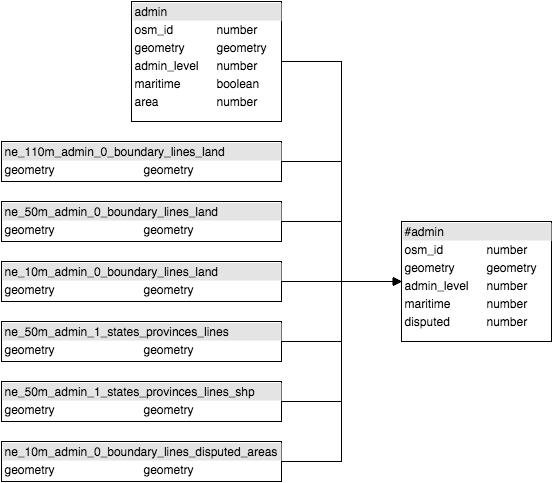
\includegraphics[scale=0.6]{images/admin_layer.png}
  \caption{Layers for administrative areas}
\end{figure}

\newpage
\subsection{Roads, Bridges and Tunnels}
Roads are split up into normal roads, tunnels and bridges after a certain zoom level. \texttt{z\_order} and \texttt{layer} attributes are used to order the geometries on the right z axis.

\begin{figure}[h]
  \centering
  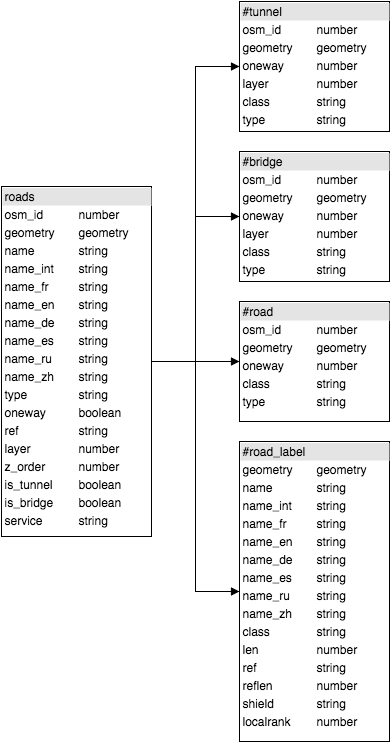
\includegraphics[scale=0.6]{images/road_layer.png}
  \caption{Layers for roads, tunnels and bridges}
\end{figure}

\newpage
\subsection{Points of Interest}
Most POIs are in fact points, but buildings tagged with POI attributes
are often polygons, which is why we need to create tables for both points and polygons.
The \texttt{localrank} and \texttt{scalerank} of the \texttt{\#poi\_label} layer are calculated from the \texttt{type} and \texttt{area} attributes.
The \texttt{address} field is pulled together from the various address attributes on the tables (\texttt{street}, \texttt{housenumber}, \texttt{place}, \texttt{city}, \texttt{postcode} and \texttt{country}).

\begin{figure}[h]
  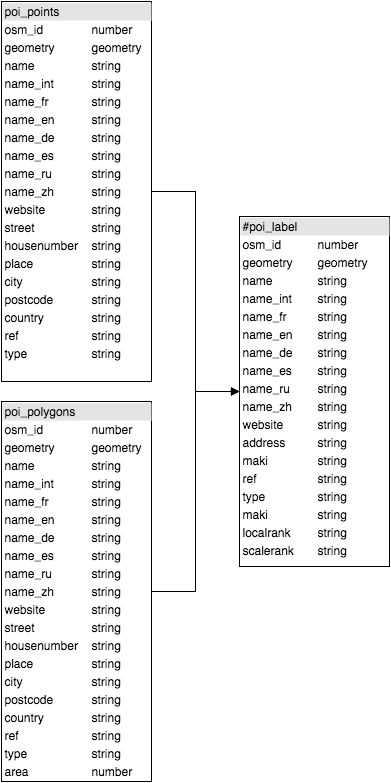
\includegraphics[scale=0.6]{images/poi_layer.png}
  \caption{Point of interest label layer}
\end{figure}

\newpage
\subsection{Water}
Water bodies for lower zoom levels are taken from Natural Earth
data while lakes and rivers are from \osm{}.

\begin{figure}[h]
  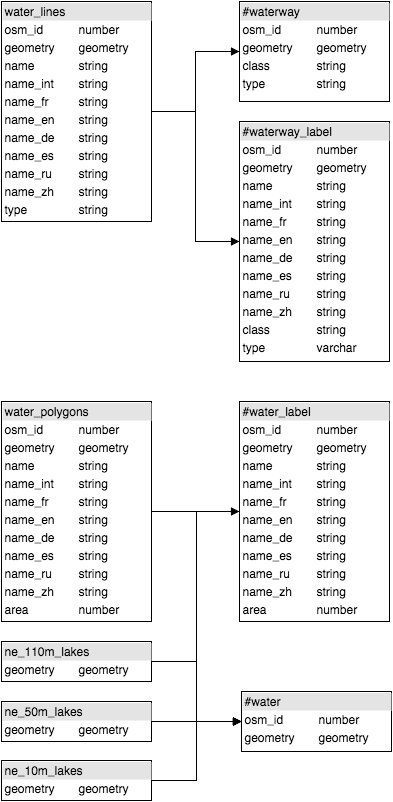
\includegraphics[scale=0.6]{images/water_layer.png}
  \caption{Water bodies and river layers}
\end{figure}

\newpage
\subsection{Places}
The original \osm{} place data is enriched with scalerank data
from Natural Earth.

\begin{figure}[h]
  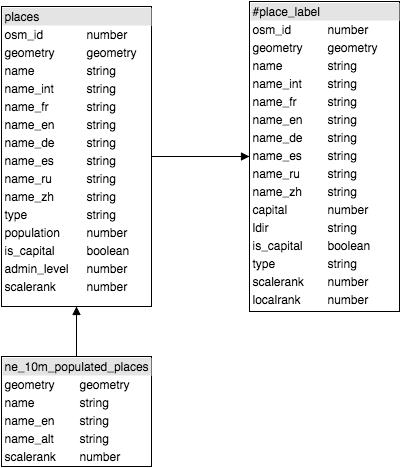
\includegraphics[scale=0.6]{images/place_layer.png}
  \caption{Place label layer}
\end{figure}